\documentclass[11pt, oneside]{article}   	% use "amsart" instead of "article" for AMSLaTeX format
\usepackage{geometry}                		% See geometry.pdf to learn the layout options. There are lots.
\geometry{letterpaper}                   		% ... or a4paper or a5paper or ... 
%\geometry{landscape}                		% Activate for for rotated page geometry
%\usepackage[parfill]{parskip}    		% Activate to begin paragraphs with an empty line rather than an indent
\usepackage{graphicx}				% Use pdf, png, jpg, or eps� with pdflatex; use eps in DVI mode
								% TeX will automatically convert eps --> pdf in pdflatex		
\usepackage{amssymb}
\usepackage{amsmath}

\title{More about e}
%\author{The Author}
\date{}							% Activate to display a given date or no date

\graphicspath{{/Users/telliott_admin/Dropbox/Tex/png/}}

\usepackage{listings,relsize} 
\lstloadlanguages{R} 
\lstset{language=R,basicstyle=\smaller[1],commentstyle=\rmfamily\smaller, 
  showstringspaces=false,% 
  xleftmargin=4ex,literate={<-}{{$\leftarrow$}}1 {~}{{$\sim$}}1} 
\lstset{escapeinside={(*}{*)}}   % for (*\ref{ }*) inside lstlistings (S code) 
\begin{document}

\maketitle
%\section{}
% \subsection*{R code}
% \begin{lstlisting}  \end{lstlisting}
% \begin{center} 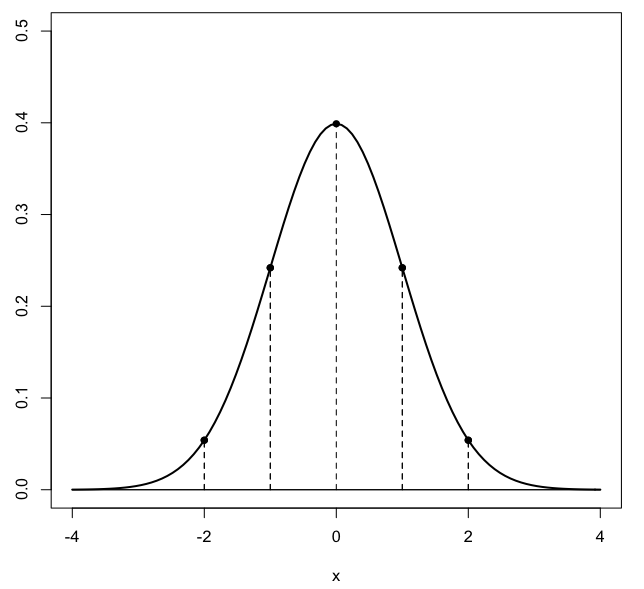
\includegraphics [scale=0.4] {gauss3.png} \end{center}
% \begin{bmatrix} a  &  b \\ c  &  d \end{bmatrix}
% \bigg |_

\large
\noindent In other write-ups I introduced $e$ as  
\[ e = \lim_{n \to \infty} (1 + \frac{1}{n})^{n} \]
and
\[ e^x = \lim_{n \to \infty} (1 + \frac{1}{n})^{nx} = \lim_{n \to \infty} (1 + \frac{x}{n})^{n} \]
From this, I derived the infinite series for $e$ and $e^x$ using the Binomial Theorem
\[ e^x = \frac{x^{0}}{0!} + \frac{x^{1}}{1!} + \frac{x^{2}}{2!} + \frac{x^{3}}{3!} + \cdots  = \sum_{k=0}^{\infty} \frac{x^{k}}{k!} \]
and I showed that 
\[ \frac{d}{dx} e^x = e^x \] 
makes complete sense in terms of the series, although we didn't actually prove it.  Starting from this, one can prove that
\[ \ln(x) = \int \frac{1}{x} \ dx \]
I saw a couple of videos on Khan academy that show how to go the other way.  So first, we will prove that 
\[ \frac{d}{dx} \ln(x) = \frac{1}{x} \]
We use our basic definition for the slope of the tangent to the curve $f(x)$
\[ \frac{d}{dx} \ln(x) = \lim_{h \to 0} \ \frac{1}{h} (\ln(x+h) - \ln(x)) \]
using
\[ log(a) - log(b) = log(\frac{a}{b}) \]
then
\[ \lim_{h \to 0} \ \frac{1}{h} (\ln(x+h) - \ln(x)) \] 
\[ \lim_{h \to 0} \ \frac{1}{h} [ \ \ln\frac{(x+h)}{x} \ ] \]
\[ = \lim_{h \to 0} \ \frac{1}{h}  \ln (1 + \frac{h}{x}) \]
using
\[ log \ ((a^b)^c) = c \ log(a^b) \]
\[  \lim_{h \to 0} \ \ln (1 + \frac{h}{x})^{1/h} \]
Substitute
\[ u = \frac{h}{x}, \ \ xu = h,  \ \ \frac{1}{xu} = \frac{1}{h} \]
and the new limit is $\lim {u \to 0}$ instead of $\lim {h \to 0}$
\[ = \lim_{u \to 0} \ \ln ((1 + u)^{1/xu}) \]
using
\[ a^{bc} = (a^b)^c \]
\[ = \lim_{u \to 0} \ \ln (((1 + u)^{1/u})^{1/x}) \]
and again, using
\[ log \ ((a^b)^c) = c \ log(a^b) \]
we have
\[ = \lim_{u \to 0} \ \frac{1}{x} \ \ln ((1 + u)^{1/u}) \]
Since $x$ isn't involved in the limit (only $h$ is changing)
\[ = \frac{1}{x} \ \lim_{u \to 0} \ \ln ((1 + u)^{1/u}) = \frac{1}{x} \ \ln (e) = \frac{1}{x} \]
\begin{equation}
  \boxed{\frac{d}{dx} \ln(x) = \frac{1}{x} }
\end{equation}
The second thing we want to do is to go on from this to show that the derivative of the function $f(x) = e^x$ is itself.  Start with
\[ \frac{d}{dx} \ln(e^x) \]
since $\ln(e^x) = x$
\[ \frac{d}{dx} \ln(e^x) = \frac{d}{dx} x = 1 \]
but using the property we just proved and the chain rule, this is also
\[ \frac{d}{dx} \ln(e^x) = \frac{1}{e^x} \ \frac{d}{dx} e^x  \]
so these two expressions are equal
\[ \frac{1}{e^x} \ \frac{d}{dx} e^x = 1  \] 
\begin{equation}
  \boxed{\frac{d}{dx} e^x = e^x }
\end{equation}


\end{document}  